\item An aircraft loops the loop of radius \( R = 500 \text{ m} \) with a constant velocity \( v = 360 \text{ km per hour} \). Find the weight of the flyer of mass \( m = 70 \text{ kg} \) in the lower, upper, and middle points of the loop.
    \begin{center}
        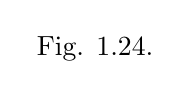
\begin{tikzpicture}
            \node at (0, 0) {Fig. 1.24.};
        \end{tikzpicture}
    \end{center}
\begin{solution}
    \begin{center}
        \begin{tikzpicture}
            \pic at (0, 0) {frame=3cm};
        \end{tikzpicture}
    \end{center}
    
    \begin{align*}
        \intertext{While moving in a loop, normal reaction exerted by the flyer on the loop at different points and uncompensated weight if any contribute to the weight of flyer at those points.}
        \intertext{(a) When the aircraft is at the lowermost point, Newton's second law of motion in projection form, \(F_n = mw_n\) gives}
        N - mg &= \dfrac{mv^2}{R} \tag{1}\\
        N &= mg + \dfrac{mv^2}{R} \tag{2}\\
           &= 2.09\, \text{kN} \tag{3}
        \intertext{(b) When it is at the upper most point, again from \(F_n = mw_n\) we get}
        N'' + mg &= \dfrac{mv^2}{R} \tag{4}\\
        N'' &= \dfrac{mv^2}{R} - mg \tag{5}\\
           &= 0.7\, \text{kN} \tag{6}
        \intertext{(c) When the aircraft is at the middle point of the loop, again from \(F_n = mw_n\)}
        N' &= \dfrac{mv^2}{R} \tag{7}\\
           &= 1.4\, \text{kN} \tag{8}
        \intertext{The uncompensated weight is \(mg\). Thus effective weight = \(\sqrt{N'^2 + m^2g^2} = 1.56\, \text{kN}\)}
    \end{align*}
\end{solution}
